% sizes tiny scriptsize footnotesize small normalsize large Large LARGE huge Huge

\documentclass[presentation]{beamer}

\usetheme{JuanLesPins}
\usecolortheme{orchid}
\setbeamertemplate{headline}{}
\setbeamertemplate{navigation symbols}{}

\usepackage{subfig}
\usepackage{graphicx}
\usepackage[english]{babel}
\usepackage[latin1]{inputenc}
\usepackage{color}
\usepackage{listings}
\input{listing_theme.tex}

\usepackage{tikz}
\usetikzlibrary{shapes}


% Add any additional packages you use in your presentation
% -----pack
% \usepackage{xxx}
% -----

% Add your custom definitions etc., if required
% -----misc
% \newcommand{\xxx}[1]{[#1]}
% -----




\title{Generational Garbage Collector}
\author{Michal Makson, Rafal Gawel}
\institute{AGH}
\date{}


\begin{document}

\begin{frame}
  \titlepage
\end{frame}

\begin{frame}{Garbage Collector}
Garbage Collector is form of automatic memory management.
Its responsibility is to reclaim memory used to allocate objects that are no longer used.
\end{frame}

\begin{frame}{Weak generational hypothesis}
	Most allocated objects die young
	
	Objects tend to live longer past a certain age
\end{frame}

\begin{frame}{Lifetime of Objects}
Add chart...
\end{frame}

\begin{frame}{Disadvantages of garbage collector}
	
	- Consuming additional resources
	- Garbage collection process impacts performance
	- Possibility of stalls in program execution
	
\end{frame}

\begin{frame}{Improving performance of Garbage Collector}
	
	Considering the fact disadvantages of using garbage collector concern mainly performance an optimization for process was searched.
	
	The solution is Generational Garbage Collector which exploits the facts from "Weak generational hypothesis"
	
\end{frame}


\begin{frame}{Generational Garbage Collection}
	Generational garbage collection algorithms are fastest and most efficient known garbage collection algorithms which make us assumptions: 
	- Heap memory is divided into older and newer objects
	- Most of the time garbage collection process runs only on newer objects
	- Collection of older objects is processed only when necessary
	
\end{frame}

\begin{frame}{Memory division}
	Except older and newer objects memory blocks, there is a third region of memory - program data area.
	To activate garbage collection process only on newer objects a simple trick is used.
	The trick is to consider older objects memory blocks as part of program data area.
\end{frame}

\begin{frame}{Pointers to Newer objects}
	To improve garbage collection process on newer objects even further the fact that vast majority of pointers to newer chunks is located in newer objects memory.
	Some of the algorithms store pointers located in old objects memory and program data to avoid scanning for them during garbage collection process.
\end{frame}

\begin{frame}{Full garbage collection processes}
	
	Garbage collection processes run on whole heap memory are only a small percentage of all generational garbage collection processes.
	Full garbage collection is executed when insufficient 
	amount of memory has been freed and to retrieve unreachable chunks.
\end{frame}

\begin{frame}{Older objects threshold}
	Generational garbage collection algorithms differ in partition between newer and older objects.
	Exact difference between older and younger object, amount of generations and frequency of full memory garbage collection differ between algorithms.
	They also make use chunk usage statistics to exploit it.
\end{frame}


\begin{frame}
By example of Java Heap fraction Eden, survivors..
\end{frame}

\begin{frame}{Mark and Sweep}{Generational collector}
content...
\end{frame}

\begin{frame}{Before a generational Minor Collection}
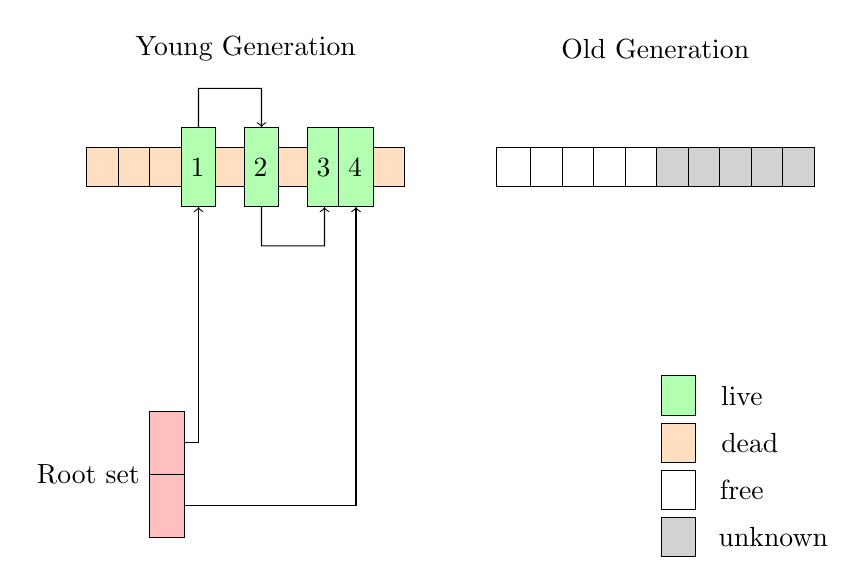
\begin{tikzpicture}
\node[xshift=2cm] {Young Generation};
\node[yshift=-1.5cm,xshift=0.2cm,draw, rectangle,fill=orange!25,text width=0.2cm, minimum height=0.5cm] {};
\node[yshift=-1.5cm,xshift=0.6cm,draw, rectangle,fill=orange!25,text width=0.2cm, minimum height=0.5cm] {};
\node[yshift=-1.5cm,xshift=1cm,draw, rectangle,fill=orange!25,text width=0.2cm, minimum height=0.5cm] {};
\node[yshift=-1.5cm,xshift=1.8cm,draw, rectangle,fill=orange!25,text width=0.2cm, minimum height=0.5cm] (3) {};
\node[yshift=-1.5cm,xshift=2.6cm,draw, rectangle,fill=orange!25,text width=0.2cm, minimum height=0.5cm] {};
\node[yshift=-1.5cm,xshift=3.8cm,draw, rectangle,fill=orange!25,text width=0.2cm, minimum height=0.5cm] {};
\node[yshift=-1.5cm,xshift=1.4cm,draw, rectangle,fill=green!30,text width=0.2cm, minimum height=1cm] (1) {1};
\node[yshift=-1.5cm,xshift=2.2cm,draw, rectangle,fill=green!30,text width=0.2cm, minimum height=1cm] (2) {2};
\node[yshift=-1.5cm,xshift=3cm,draw, rectangle,fill=green!30,text width=0.2cm, minimum height=1cm] (3) {3};
\node[yshift=-1.5cm,xshift=3.4cm,draw, rectangle,fill=green!30,text width=0.2cm, minimum height=1cm] (4) {4};


\node[xshift=7.2cm] () {Old Generation};
\node[yshift=-1.5cm,xshift=9cm,draw, rectangle,fill=gray!35,text width=0.2cm, minimum height=0.5cm] {};
\node[yshift=-1.5cm,xshift=8.6cm,draw, rectangle,fill=gray!35,text width=0.2cm, minimum height=0.5cm] {};
\node[yshift=-1.5cm,xshift=8.2cm,draw, rectangle,fill=gray!35,text width=0.2cm, minimum height=0.5cm] {};
\node[yshift=-1.5cm,xshift=7.8cm,draw, rectangle,fill=gray!35,text width=0.2cm, minimum height=0.5cm] {};
\node[yshift=-1.5cm,xshift=7.4cm,draw, rectangle,fill=gray!35,text width=0.2cm, minimum height=0.5cm] {};
\node[yshift=-1.5cm,xshift=7cm,draw, rectangle,fill=white,text width=0.2cm, minimum height=0.5cm] {};
\node[yshift=-1.5cm,xshift=6.6cm,draw, rectangle,fill=white,text width=0.2cm, minimum height=0.5cm] {};
\node[yshift=-1.5cm,xshift=6.2cm,draw, rectangle,fill=white,text width=0.2cm, minimum height=0.5cm] {};
\node[yshift=-1.5cm,xshift=5.8cm,draw, rectangle,fill=white,text width=0.2cm, minimum height=0.5cm] {};
\node[yshift=-1.5cm,xshift=5.4cm,draw, rectangle,fill=white,text width=0.2cm, minimum height=0.5cm] {};

\node[yshift=-4.4cm,xshift=8.3cm] {live};
\node[yshift=-4.4cm,xshift=7.5cm,draw, rectangle,fill=green!30,text width=0.2cm, minimum height=0.5cm] {};
\node[yshift=-5cm,xshift=8.4cm] {dead};
\node[yshift=-5cm,xshift=7.5cm,draw, rectangle,fill=orange!25,text width=0.2cm, minimum height=0.5cm] {};
\node[yshift=-5.6cm,xshift=8.3cm] {free};
\node[yshift=-5.6cm,xshift=7.5cm,draw, rectangle,fill=white,text width=0.2cm, minimum height=0.5cm] {};
\node[yshift=-6.2cm,xshift=8.7cm] {unknown};
\node[yshift=-6.2cm,xshift=7.5cm,draw, rectangle,fill=gray!35,text width=0.2cm, minimum height=0.5cm] {};

\node[yshift=-5.4cm] {Root set};
\node[xshift=1cm,yshift=-5cm,draw, rectangle,fill=red!25,text width=0.2cm, minimum height=0.8cm] (R1) {};
\node[xshift=1cm,yshift=-5.8cm,draw, rectangle,fill=red!25,text width=0.2cm, minimum height=0.8cm] (R2) {};
\draw[->, to path={-| (\tikztotarget)}] (R1) edge (1);
\draw[->, to path={-| (\tikztotarget)}] (R2) edge (4);
\draw[->] (1) -- (1.4,-0.5) -- (2.2,-0.5) -> (2);
\draw[->] (2) -- (2.2,-2.5) -- (3,-2.5) -> (3);
\end{tikzpicture}
\end{frame}

\begin{frame}{After a generational Minor Collection}
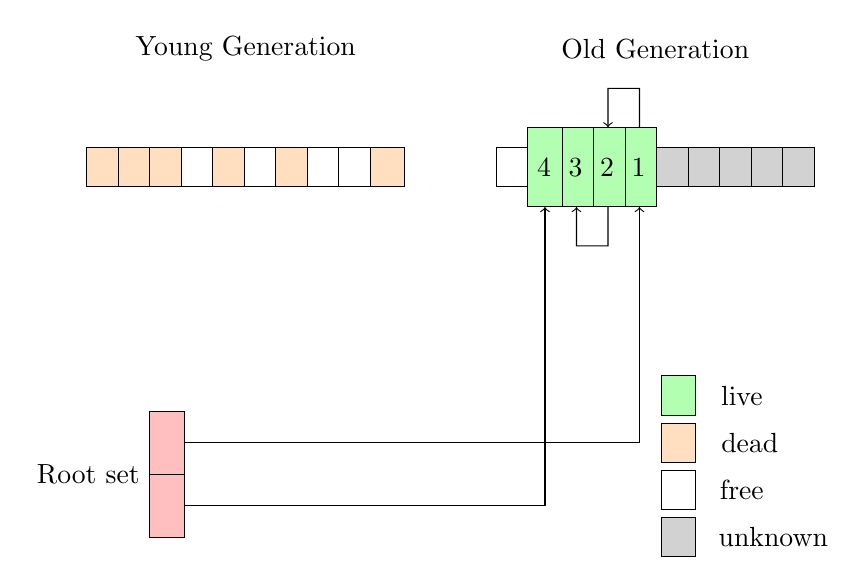
\begin{tikzpicture}
\node[xshift=2cm] {Young Generation};
\node[yshift=-1.5cm,xshift=0.2cm,draw, rectangle,fill=orange!25,text width=0.2cm, minimum height=0.5cm] {};
\node[yshift=-1.5cm,xshift=0.6cm,draw, rectangle,fill=orange!25,text width=0.2cm, minimum height=0.5cm] {};
\node[yshift=-1.5cm,xshift=1cm,draw, rectangle,fill=orange!25,text width=0.2cm, minimum height=0.5cm] {};
\node[yshift=-1.5cm,xshift=1.4cm,draw, rectangle,fill=white,text width=0.2cm, minimum height=0.5cm] {};
\node[yshift=-1.5cm,xshift=1.8cm,draw, rectangle,fill=orange!25,text width=0.2cm, minimum height=0.5cm] (3) {};
\node[yshift=-1.5cm,xshift=2.2cm,draw, rectangle,fill=white,text width=0.2cm, minimum height=0.5cm] {};
\node[yshift=-1.5cm,xshift=2.6cm,draw, rectangle,fill=orange!25,text width=0.2cm, minimum height=0.5cm] {};
\node[yshift=-1.5cm,xshift=3cm,draw, rectangle,fill=white,text width=0.2cm, minimum height=0.5cm] {};
\node[yshift=-1.5cm,xshift=3.4cm,draw, rectangle,fill=white,text width=0.2cm, minimum height=0.5cm] {};
\node[yshift=-1.5cm,xshift=3.8cm,draw, rectangle,fill=orange!25,text width=0.2cm, minimum height=0.5cm] {};





\node[xshift=7.2cm] () {Old Generation};
\node[yshift=-1.5cm,xshift=9cm,draw, rectangle,fill=gray!35,text width=0.2cm, minimum height=0.5cm] {};
\node[yshift=-1.5cm,xshift=8.6cm,draw, rectangle,fill=gray!35,text width=0.2cm, minimum height=0.5cm] {};
\node[yshift=-1.5cm,xshift=8.2cm,draw, rectangle,fill=gray!35,text width=0.2cm, minimum height=0.5cm] {};
\node[yshift=-1.5cm,xshift=7.8cm,draw, rectangle,fill=gray!35,text width=0.2cm, minimum height=0.5cm] {};
\node[yshift=-1.5cm,xshift=7.4cm,draw, rectangle,fill=gray!35,text width=0.2cm, minimum height=0.5cm] {};
\node[yshift=-1.5cm,xshift=5.4cm,draw, rectangle,fill=white,text width=0.2cm, minimum height=0.5cm] {};
\node[yshift=-1.5cm,xshift=7cm,draw, rectangle,fill=green!30,text width=0.2cm, minimum height=1cm] (1) {1};
\node[yshift=-1.5cm,xshift=6.6cm,draw, rectangle,fill=green!30,text width=0.2cm, minimum height=1cm] (2) {2};
\node[yshift=-1.5cm,xshift=6.2cm,draw, rectangle,fill=green!30,text width=0.2cm, minimum height=1cm] (3) {3};
\node[yshift=-1.5cm,xshift=5.8cm,draw, rectangle,fill=green!30,text width=0.2cm, minimum height=1cm] (4) {4};

\node[yshift=-4.4cm,xshift=8.3cm] {live};
\node[yshift=-4.4cm,xshift=7.5cm,draw, rectangle,fill=green!30,text width=0.2cm, minimum height=0.5cm] {};
\node[yshift=-5cm,xshift=8.4cm] {dead};
\node[yshift=-5cm,xshift=7.5cm,draw, rectangle,fill=orange!25,text width=0.2cm, minimum height=0.5cm] {};
\node[yshift=-5.6cm,xshift=8.3cm] {free};
\node[yshift=-5.6cm,xshift=7.5cm,draw, rectangle,fill=white,text width=0.2cm, minimum height=0.5cm] {};
\node[yshift=-6.2cm,xshift=8.7cm] {unknown};
\node[yshift=-6.2cm,xshift=7.5cm,draw, rectangle,fill=gray!35,text width=0.2cm, minimum height=0.5cm] {};

\node[yshift=-5.4cm] {Root set};
\node[xshift=1cm,yshift=-5cm,draw, rectangle,fill=red!25,text width=0.2cm, minimum height=0.8cm] (R1) {};
\node[xshift=1cm,yshift=-5.8cm,draw, rectangle,fill=red!25,text width=0.2cm, minimum height=0.8cm] (R2) {};
\draw[->, to path={-| (\tikztotarget)}] (R1) edge (1);
\draw[->, to path={-| (\tikztotarget)}] (R2) edge (4);
\draw[->] (1) -- (7,-0.5) -- (6.6,-0.5) -> (2);
\draw[->] (2) -- (6.6,-2.5) -- (6.2,-2.5) -> (3);
\end{tikzpicture}
\end{frame}

\end{document}
